\section{问题三的模型建立与求解}\label{sec:model3}

\subsection{系统偏差存在性检验}

附件3为真实测量数据，需判断是否存在系统偏差。采用\textbf{双判据}策略：

\textbf{（1）Wald 检验}\cite{wald1943}。在联合估计框架下估得 $(\hat{\Delta\tau}, \hat{\Delta x}, \hat{\Delta y})$ 及其 Bootstrap\cite{efron1979} 协方差 $\hat{\boldsymbol{\Sigma}}$，构造统计量：
\begin{equation}
    W = (\hat{\Delta x}, \hat{\Delta y}) \hat{\boldsymbol{\Sigma}}^{-1} (\hat{\Delta x}, \hat{\Delta y})^\top \sim \chi^2(2)
\end{equation}

\textbf{（2）AIC 对比}\cite{akaike1974}。比较零偏模型（仅含 $\Delta\tau$，1 参数）与带偏模型（含 $\Delta\tau, \Delta x, \Delta y$，3 参数）：
\begin{equation}
    \text{AIC} = n \ln(\text{SSE}/n) + 2k
\end{equation}

判决规则：当 Wald $p < 0.05$ \textbf{且} $\Delta\text{AIC} > 2$ 时接受 H$_1$（有偏差），否则接受 H$_0$。

\begin{algorithm}[htbp]
\caption{系统偏差存在性检验与融合算法（问题三）}
\label{alg:p3_test}
\KwIn{方式1数据 $\{\boldsymbol{z}_1^k, t_1^k\}$，方式2数据 $\{\boldsymbol{z}_2^k, t_2^k\}$}
\KwOut{判决结果（有偏/无偏）、融合轨迹 $\{\hat{\boldsymbol{p}}(0.1k)\}$}

\tcp{步骤1：联合估计（带偏模型）}
用 Nelder-Mead 最小化式~\eqref{eq:p2_joint} 得 $(\hat{\Delta\tau}, \hat{\Delta x}, \hat{\Delta y})$ \\
计算带偏模型残差平方和 $\text{SSE}_1$

\tcp{步骤2：Bootstrap 估计协方差矩阵}
\For{$b = 1, 2, \ldots, 200$}{
    重采样数据（分层 Bootstrap，保持时序结构） \\
    重估参数得 $(\Delta\tau^{(b)}, \Delta x^{(b)}, \Delta y^{(b)})$
}
计算样本协方差 $\hat{\boldsymbol{\Sigma}} \leftarrow \text{cov}(\{(\Delta x^{(b)}, \Delta y^{(b)})\})$

\tcp{步骤3：Wald 检验}
构造统计量 $W = (\hat{\Delta x}, \hat{\Delta y}) \hat{\boldsymbol{\Sigma}}^{-1} (\hat{\Delta x}, \hat{\Delta y})^\top$ \\
计算 $p$-value：$p_W \leftarrow P(\chi^2(2) > W)$ \tcp*{自由度2}

\tcp{步骤4：AIC 对比}
用一维搜索估计零偏模型（仅 $\Delta\tau$）得 $\hat{\Delta\tau}_0$，计算 $\text{SSE}_0$ \\
$n \leftarrow$ 公共时段观测点数 \\
$\text{AIC}_0 \leftarrow n \ln(\text{SSE}_0/n) + 2 \times 1$ \tcp*{零偏模型：1参数}
$\text{AIC}_1 \leftarrow n \ln(\text{SSE}_1/n) + 2 \times 3$ \tcp*{带偏模型：3参数}
$\Delta\text{AIC} \leftarrow \text{AIC}_0 - \text{AIC}_1$

\tcp{步骤5：双判据判决}
\eIf{$p_W < 0.05$ \textbf{且} $\Delta\text{AIC} > 2$}{
    判决 $\leftarrow$ H$_1$（存在系统偏差） \\
    执行卡尔曼融合（同算法~\ref{alg:p2_kf}，使用 $\hat{\Delta x}, \hat{\Delta y}$ 校正）
}{
    判决 $\leftarrow$ H$_0$（无系统偏差） \\
    执行卡尔曼融合（使用 $\hat{\Delta\tau}_0$，不校正空间偏差）
}

\tcp{步骤6：输出融合轨迹}
按选定模型执行异步卡尔曼滤波，输出 10\,Hz 轨迹
\end{algorithm}

\begin{figure}[H]
    \centering
    \begin{tikzpicture}[node distance=0.4cm,
        sbox/.style={rectangle, draw=black!80, thick, fill=black!4, minimum width=14em, minimum height=2em, align=center, font=\small, rounded corners=2pt, blur shadow={shadow blur steps=5, shadow xshift=0.3mm, shadow yshift=-0.3mm}},
        dec/.style={diamond, draw=black!80, thick, fill=black!7, aspect=2.5, minimum width=7em, align=center, font=\small, inner sep=1pt},
        res/.style={rectangle, rounded corners=4pt, draw=black!80, thick, fill=black!12, minimum width=11em, minimum height=1.8em, align=center, font=\small\bfseries},
        param/.style={font=\scriptsize, text=black!55},
        arr/.style={-Stealth, thick, black!70}]

        \node[sbox] (s1) {带偏模型估计 $(\Delta\tau, \Delta x, \Delta y)$};
        \node[sbox, below=of s1] (s2) {零偏模型估计 $(\Delta\tau)$};
        \node[sbox, below=of s2] (s3) {Bootstrap 协方差 $\hat{\Sigma}$ ($n=1000$)};
        \node[dec, below=0.8cm of s3] (d1) {$p < 0.05$\,\textbf{且}\,$\Delta$AIC $> 2$?};
        \node[res, below left=1cm and 0.5cm of d1] (h0) {$H_0$：无偏差\\零偏模型融合};
        \node[res, below right=1cm and 0.5cm of d1] (h1) {$H_1$：有偏差\\带偏模型融合};

        \draw[arr] (s1) -- (s2);
        \draw[arr] (s2) -- (s3);
        \draw[arr] (s3) -- (d1);
        \draw[arr] (d1) -| node[pos=0.25, above, param]{否} (h0);
        \draw[arr] (d1) -| node[pos=0.25, above, param]{是} (h1);

        \node[param, right=0.5cm of s3] {$W=2.10$, $p=0.35$};
        \node[param, right=0.5cm of s1] {SSE$=28603$};
        \node[param, right=0.5cm of s2] {SSE$=28660$};
    \end{tikzpicture}
    \caption{问题三求解流程}
    \label{fig:flow_p3}
\end{figure}

\subsection{检验结果}

\begin{table}[htbp]
    \centering
    \caption{问题三偏差检验结果}
    \label{tab:p3_test}
    \begin{tabular}{@{}lrl@{}}
        \toprule
        指标 & 数值 & 判定 \\
        \midrule
        $\hat{\Delta\tau}$ & $367.8659$\,s & — \\
        $\hat{\Delta x}$ & $0.0883$\,m & 极小 \\
        $\hat{\Delta y}$ & $0.2959$\,m & 极小 \\
        Wald $W$ & 2.0659 & $p = 0.356 > 0.05$ \\
        $\Delta$AIC & $-2.81$ & $< 2$ \\
        \midrule
        \textbf{判决} & \multicolumn{2}{l}{\textbf{H$_0$：无显著系统偏差}} \\
        \bottomrule
    \end{tabular}
\end{table}

两路数据在空间上无固定偏移，仅存在时间偏差 $\Delta\tau \approx 367.87$\,s。

\subsection{KF 融合与输出}

按零偏模型执行卡尔曼滤波融合（同问题二流程，但 $\Delta x = \Delta y = 0$）。融合参数根据 EDA 估计噪声调整：$\sigma_1 \approx 4.18$\,m，$\sigma_2 \approx 2.89$\,m（噪声水平由 EDA 阶段二阶差分方法估计，详见表~\ref{fig:noise_heat} 所示噪声热力图），过程噪声 $q_a = 8$\,m/s$^2$。

输出 10\,Hz 轨迹 \textbf{3691 点}（时长 369.0\,s），作为问题四的输入。

\begin{figure}[htbp]
    \centering
    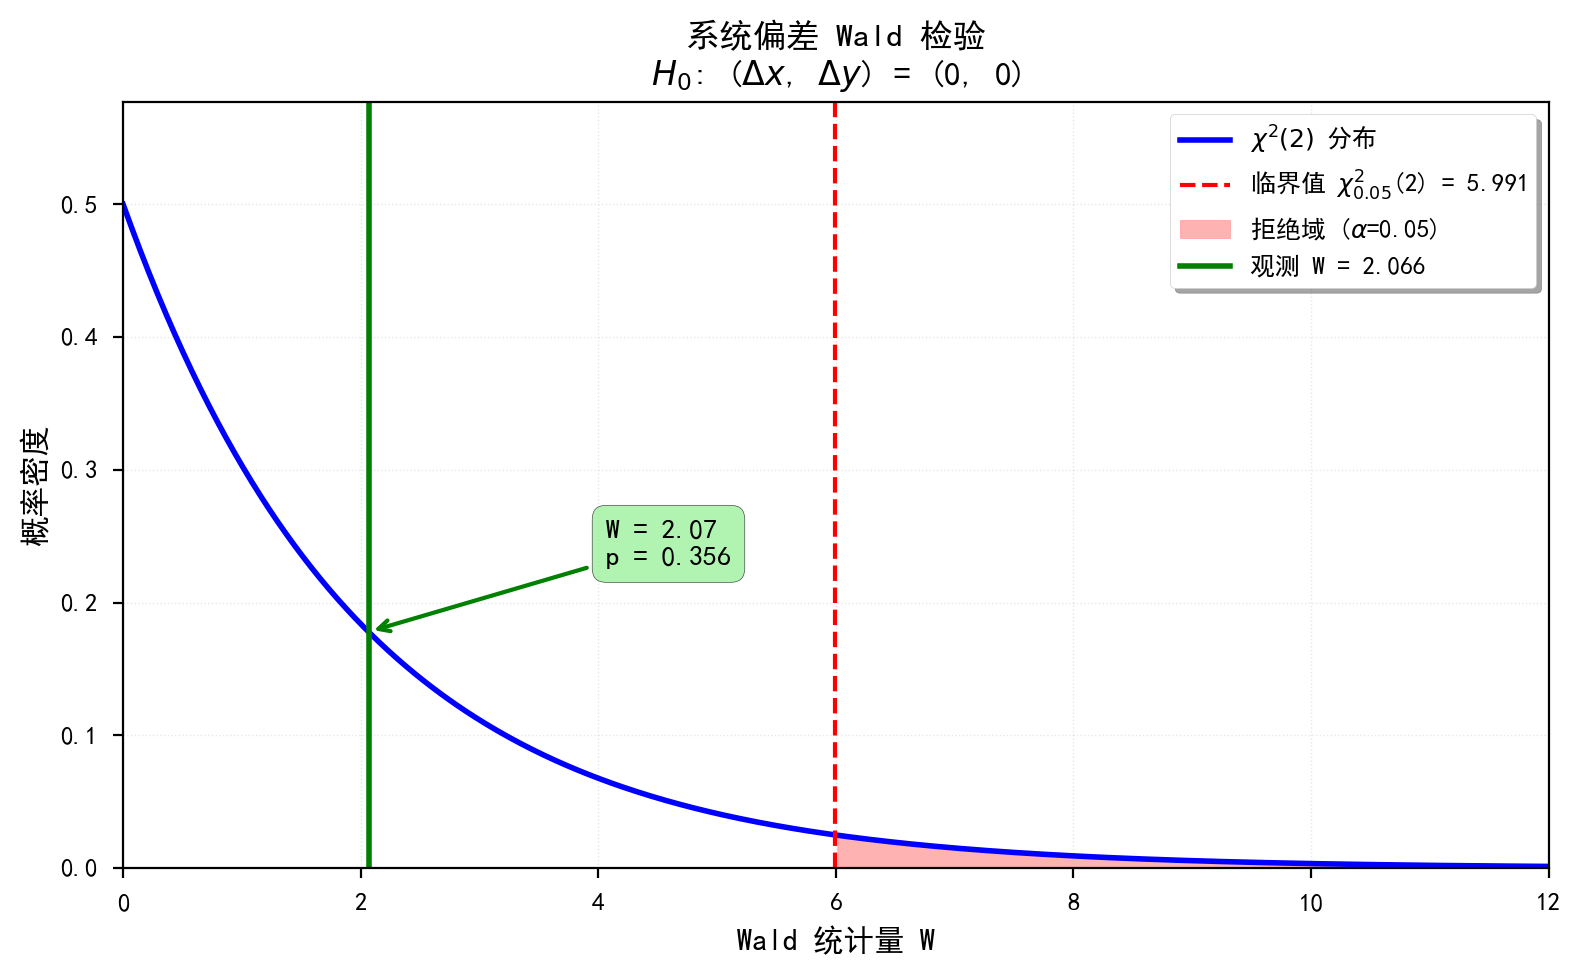
\includegraphics[width=0.7\textwidth]{figures/fig_p3_wald_chi2.png}
    \caption{Wald 检验：$\chi^2(2)$ 分布下 $W=2.07$ 远低于临界值 5.991（接受 H$_0$）}
    \label{fig:p3_wald}
\end{figure}

\begin{figure}[htbp]
    \centering
    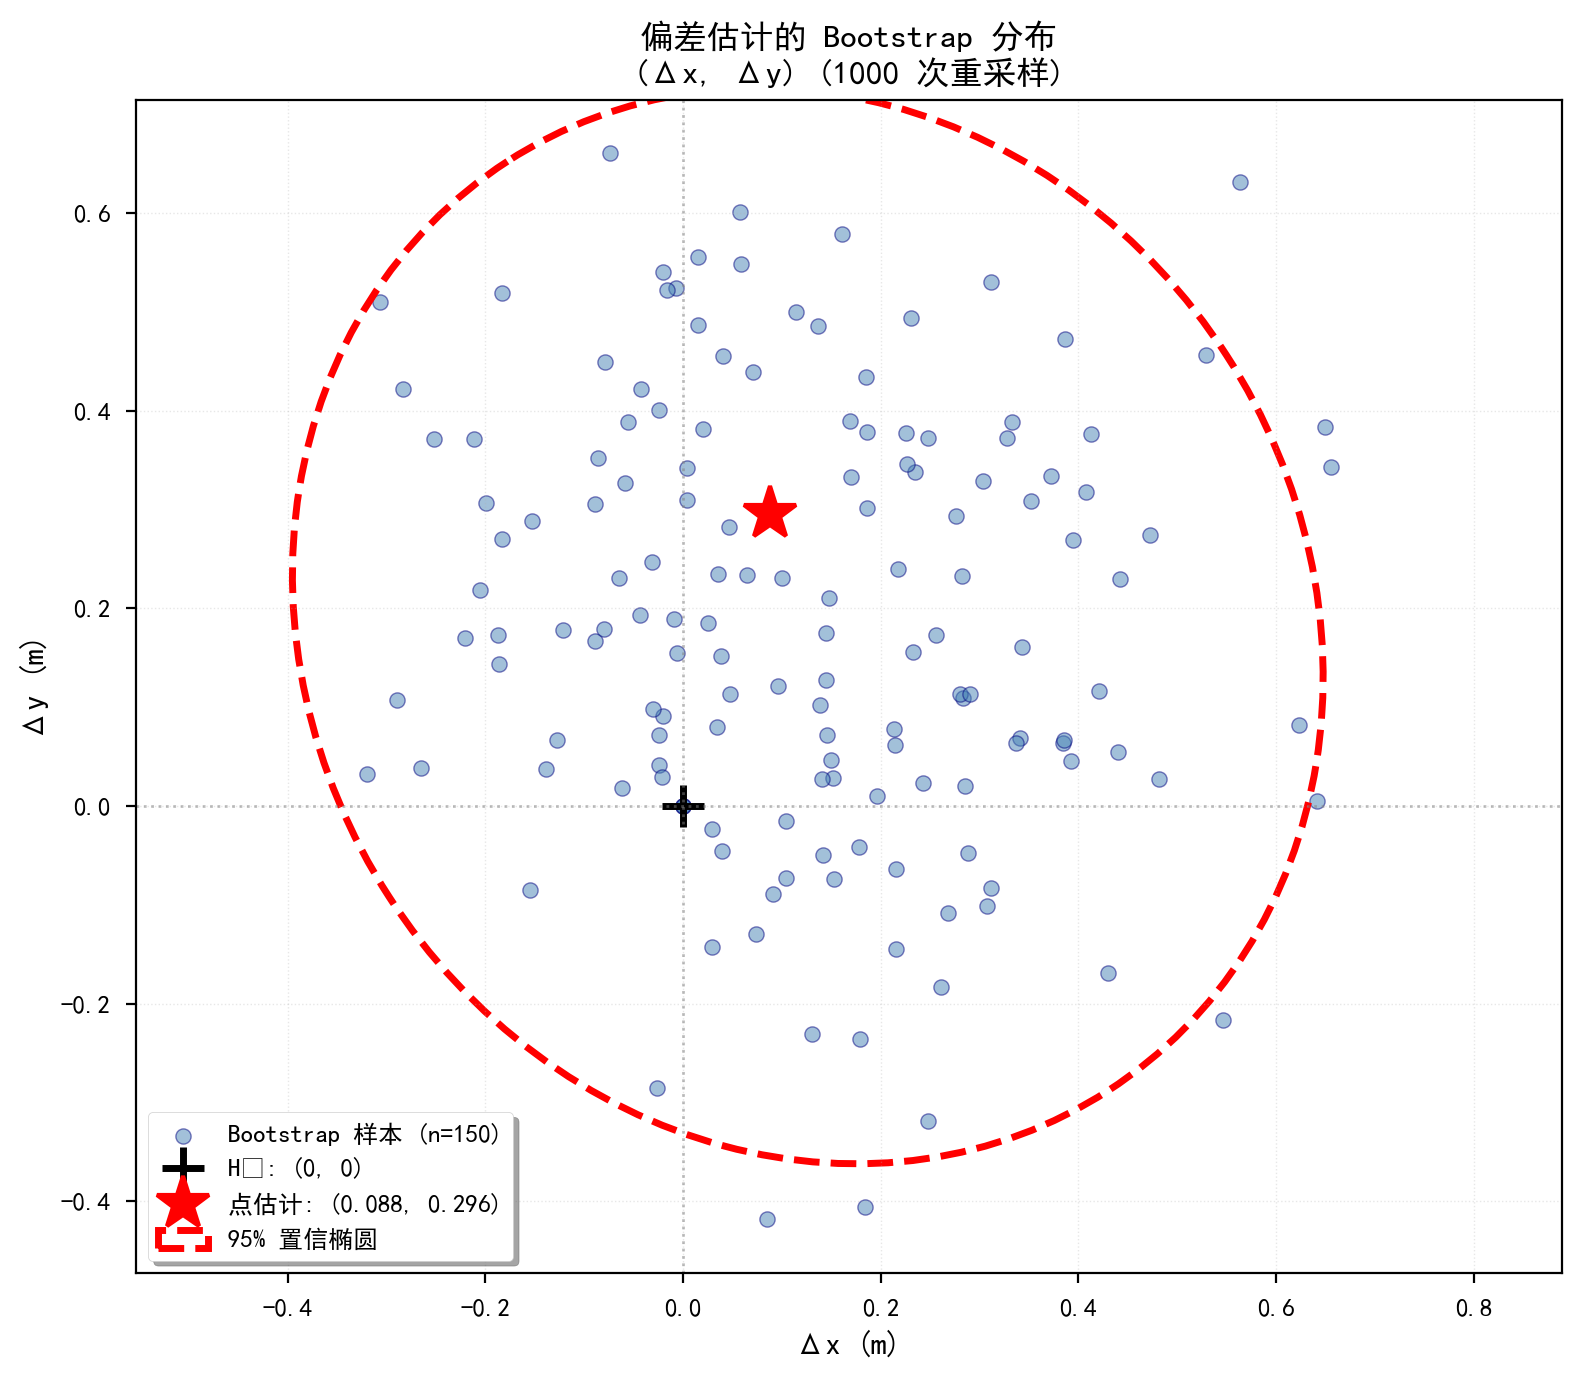
\includegraphics[width=0.65\textwidth]{figures/fig_p3_bootstrap_scatter.png}
    \caption{Bootstrap 偏差估计散点与 95\% 置信椭圆（椭圆包含原点，支持 H$_0$）}
    \label{fig:p3_bootstrap}
\end{figure}

\begin{figure}[htbp]
    \centering
    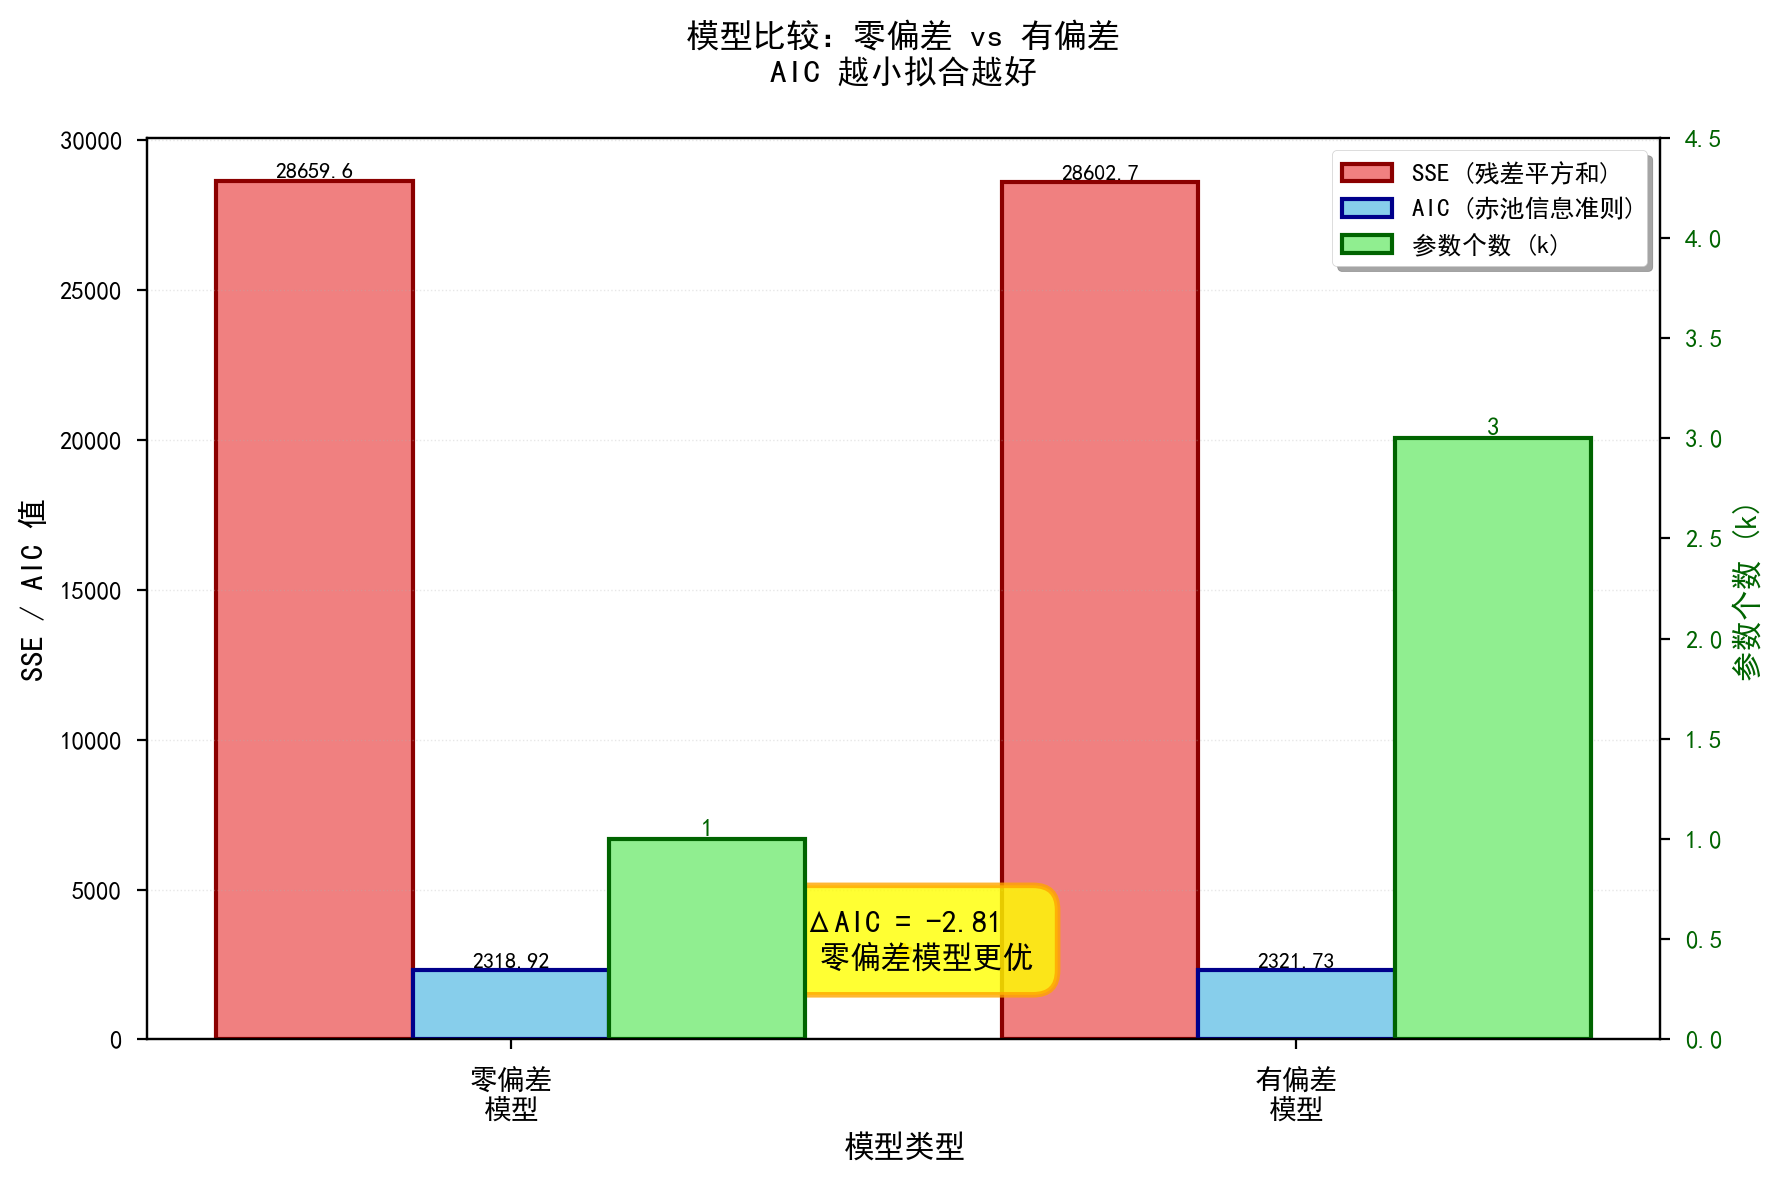
\includegraphics[width=0.7\textwidth]{figures/fig_p3_model_comparison.png}
    \caption{零偏模型 vs 带偏模型：AIC 对比（$\Delta$AIC$=-2.81$，零偏更优）}
    \label{fig:p3_aic}
\end{figure}
